\documentclass[11pt,a4paper,spanish]{book}
\usepackage{estilo_unir-1}
\hypersetup{
	colorlinks   = true,
	urlcolor     = blue,
	linkcolor    = black,
	citecolor    = red
}
\usepackage[nottoc]{tocbibind}
\usepackage{tikz}
\usetikzlibrary{shapes.geometric, arrows.meta, positioning, fit}

%---------------------------
% Datos del trabajo
%---------------------------
\subject{Pr\'{a}cticas Acad\'{e}micas Externas}
\title{Sistema de medici\'{o}n de impedancia (EIS) para cuantificaci\'{o}n de Candida albicans --- Fase 1}
\author{Andr\'{e}s Alexandro Tapia Flores}
\profesor{Universidad Internacional de la Rioja (UNIR)}
\date{Marzo 2026}

\begin{document}
\renewcommand{\listfigurename}{\'{I}ndice de figuras}
\renewcommand{\contentsname}{\'{I}ndice de contenidos}
\renewcommand{\figurename}{Figura}
\renewcommand{\tablename}{Tabla}

\maketitle
\frontmatter
\tableofcontents

\chapter{Resumen}
Este documento presenta la especificaci\'{o}n de requerimientos y el diagrama de bloques del sistema de medici\'{o}n de impedancia electroqu\'{i}mica (EIS) basado en ESP32 y AD5933, orientado a la detecci\'{o}n de \textit{Candida albicans} en muestras de saliva. Se describe la arquitectura hardware y software del sistema, se identifican las variables EIS relevantes y se definen los requerimientos funcionales para la implementaci\'{o}n en Python.

\vspace{0.5cm}
{\bf Palabras clave:} espectroscop\'{i}a de impedancia electroqu\'{i}mica, candida albicans, sistema embebido, clasificaci\'{o}n cu\'{a}ntica, esp32

\mainmatter

\chapter{Introducci\'{o}n}

El presente Trabajo corresponde a la Fase~1 del reto de pr\'{a}cticas externas, cuyo objetivo general es el dise\~{n}o e implementaci\'{o}n de un sistema de adquisici\'{o}n y an\'{a}lisis de datos de espectroscop\'{i}a de impedancia electroqu\'{i}mica (EIS) para la cuantificaci\'{o}n de \textit{Candida albicans}.

La propuesta original contemplaba el uso de LabVIEW como entorno de desarrollo. Sin embargo, se opt\'{o} por una implementaci\'{o}n en Python puro, lo que permite mayor portabilidad, integraci\'{o}n con bibliotecas de an\'{a}lisis de datos y facilidad de despliegue.

El sistema se compone de un m\'{o}dulo hardware basado en el microcontrolador ESP32 conectado al circuito integrado AD5933 (analizador de impedancia), y un backend en Python que gestiona la comunicaci\'{o}n serial, el procesamiento de datos y la visualizaci\'{o}n en tiempo real a trav\'{e}s de una interfaz web.

\section{Estructura del documento}
En la Secci\'{o}n~2 se presentan los objetivos. La Secci\'{o}n~3 describe la arquitectura del sistema mediante un diagrama de bloques. La Secci\'{o}n~4 recoge los requerimientos funcionales. Finalmente, la Secci\'{o}n~5 resume las conclusiones.


\chapter{Objetivos}

\section{Objetivo general}
Analizar y especificar los requerimientos del sistema EIS basado en ESP32 + AD5933 con software en Python para la detecci\'{o}n de \textit{Candida albicans}.

\section{Objetivos espec\'{i}ficos}
\begin{itemize}
	\item Comprender la arquitectura hardware: celda electroqu\'{i}mica, AD5933, ESP32 y protocolo de comunicaci\'{o}n serial.
	\item Identificar las variables EIS relevantes: frecuencia ($f$), parte real de la impedancia ($\mathrm{Re}(Z)$), parte imaginaria ($\mathrm{Im}(Z)$), magnitud ($|Z|$), fase ($\phi$) y temperatura.
	\item Definir los requerimientos funcionales del software.
	\item Elaborar el diagrama de bloques del sistema completo.
	\item Definir el uso de un clasificador cu\'{a}ntico variacional (VQC) para la clasificaci\'{o}n de espectros EIS.
\end{itemize}


\chapter{Arquitectura del sistema}

El sistema se estructura en tres capas principales: hardware de medici\'{o}n, backend de comunicaci\'{o}n y frontend de visualizaci\'{o}n.

\begin{figure}[h]
\centering
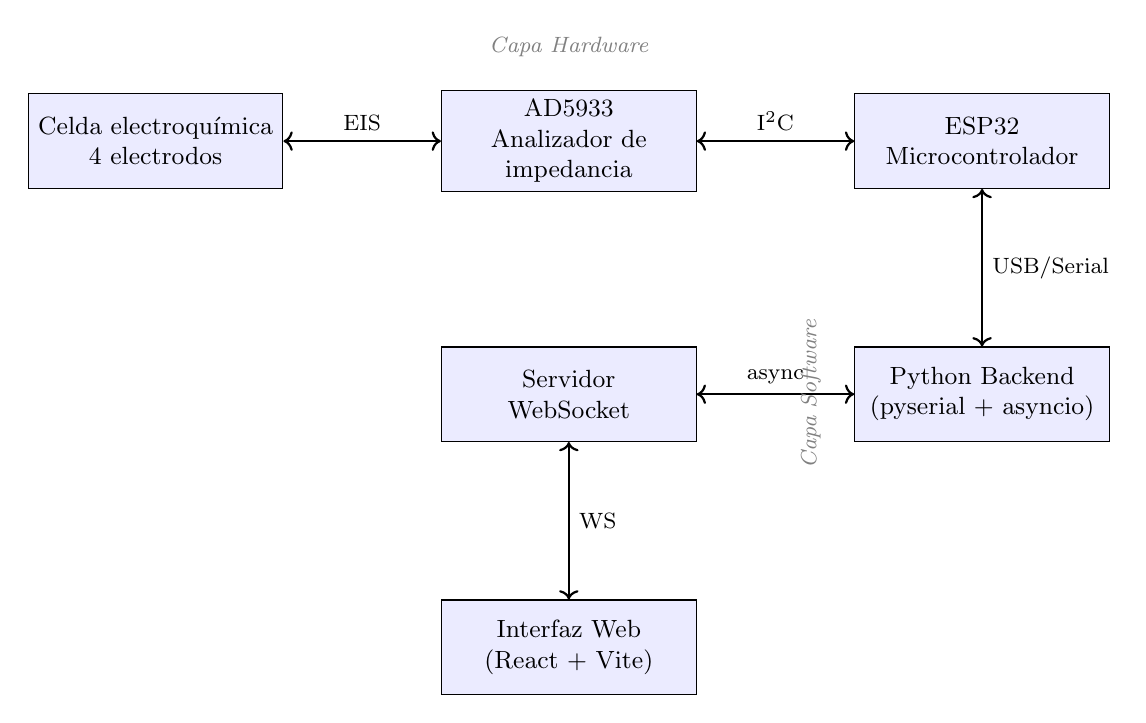
\begin{tikzpicture}[
	block/.style={rectangle, draw, fill=blue!8, text width=3cm, minimum height=1.2cm, align=center, font=\small},
	arrow/.style={-{Stealth[length=3mm]}, thick},
	node distance=1.5cm and 2cm
]
	% Hardware layer
	\node[block] (cell) {Celda electroqu\'{i}mica\\4 electrodos};
	\node[block, right=of cell] (ad5933) {AD5933\\Analizador de\\impedancia};
	\node[block, right=of ad5933] (esp32) {ESP32\\Microcontrolador};

	% Software layer
	\node[block, below=2cm of esp32] (python) {Python Backend\\(pyserial + asyncio)};
	\node[block, left=of python] (ws) {Servidor\\WebSocket};

	% Frontend
	\node[block, below=2cm of ws] (web) {Interfaz Web\\(React + Vite)};

	% Arrows
	\draw[arrow, <->] (cell) -- node[above, font=\footnotesize]{EIS} (ad5933);
	\draw[arrow, <->] (ad5933) -- node[above, font=\footnotesize]{I\textsuperscript{2}C} (esp32);
	\draw[arrow, <->] (esp32) -- node[right, font=\footnotesize]{USB/Serial} (python);
	\draw[arrow, <->] (python) -- node[above, font=\footnotesize]{async} (ws);
	\draw[arrow, <->] (ws) -- node[right, font=\footnotesize]{WS} (web);

	% Labels
	\node[above=0.3cm of ad5933, font=\footnotesize\itshape, text=gray] {Capa Hardware};
	\node[left=0.3cm of python, font=\footnotesize\itshape, text=gray, rotate=90, anchor=south] {Capa Software};
\end{tikzpicture}
\caption[Diagrama de bloques del sistema]{Diagrama de bloques del sistema EIS. La celda electroqu\'{i}mica se conecta al AD5933 que mide la impedancia. El ESP32 lee los datos v\'{i}a I\textsuperscript{2}C y los transmite por serial al backend Python, que a su vez los distribuye por WebSocket a la interfaz web. Fuente: elaboraci\'{o}n propia.}
\label{fig:bloques}
\end{figure}

\section{Capa hardware}

\begin{itemize}
	\item \textbf{Celda electroqu\'{i}mica (4 electrodos):} contenedor de 1~mL para muestras de saliva. Los cuatro electrodos permiten mediciones de impedancia precisas al separar el circuito de excitaci\'{o}n del circuito de medici\'{o}n.
	\item \textbf{AD5933:} circuito integrado analizador de impedancia de Analog Devices. Genera se\~{n}ales de excitaci\'{o}n sinusoidal y mide la respuesta en frecuencia, proporcionando las componentes real e imaginaria de la impedancia. Se comunica con el ESP32 mediante el bus I\textsuperscript{2}C.
	\item \textbf{ESP32:} microcontrolador con conectividad Wi-Fi/Bluetooth. Gestiona la comunicaci\'{o}n I\textsuperscript{2}C con el AD5933, implementa el protocolo de comandos y transmite los datos al PC mediante USB serial a 115200~baudios.
\end{itemize}

\section{Capa software}
\begin{itemize}
	\item \textbf{Collector (Python):} m\'{o}dulo que gestiona la conexi\'{o}n serial con el ESP32 usando \texttt{pyserial}. Lee las tramas JSON de datos de impedancia y distribuye los valores a los consumidores registrados.
	\item \textbf{Coordinator (Python):} servidor WebSocket as\'{i}ncrono basado en \texttt{asyncio} y \texttt{websockets}. Recibe los datos del Collector y los retransmite en tiempo real a los clientes web conectados. Tambi\'{e}n permite enviar comandos de configuraci\'{o}n al ESP32.
	\item \textbf{Interfaz web (React + Vite):} frontend que muestra los datos EIS en tiempo real mediante gr\'{a}ficos interactivos.
\end{itemize}

\section{Variables EIS identificadas}

La Tabla~\ref{tab:variables} resume las variables de inter\'{e}s del sistema.

\begin{table}[h]
	\centering
	\begin{tabular}{l l l}
		\hline\hline
		Variable & S\'{i}mbolo & Unidad \\ [0.5ex]
		\hline
		Frecuencia          & $f$              & Hz \\
		Parte real           & $\mathrm{Re}(Z)$ & $\Omega$ \\
		Parte imaginaria     & $\mathrm{Im}(Z)$ & $\Omega$ \\
		Magnitud             & $|Z|$            & $\Omega$ \\
		Fase                 & $\phi$           & grados \\
		Temperatura          & $T$              & \textdegree C \\
		\hline
	\end{tabular}
	\caption[Variables EIS del sistema]{Variables de espectroscop\'{i}a de impedancia electroqu\'{i}mica medidas por el sistema. Fuente: elaboraci\'{o}n propia.}
	\label{tab:variables}
\end{table}


\chapter{Requerimientos funcionales}

A continuaci\'{o}n se listan los requerimientos funcionales del software.

\begin{table}[h]
	\centering
	\begin{tabular}{l p{10cm}}
		\hline\hline
		ID & Descripci\'{o}n \\ [0.5ex]
		\hline
		RF-01 & El sistema debe establecer comunicaci\'{o}n serial con el ESP32 a 115200~baud. \\
		RF-02 & El sistema debe soportar los comandos: PING, CFG, CAL, START/SWEEP, STOP, TEMP. \\
		RF-03 & El sistema debe recibir y parsear tramas JSON con datos de impedancia ($f$, $\mathrm{Re}(Z)$, $\mathrm{Im}(Z)$, $|Z|$, $\phi$). \\
		RF-04 & El sistema debe permitir configurar los par\'{a}metros del barrido: $f_{\min}$, $f_{\max}$, n\'{u}mero de puntos y ciclos de estabilizaci\'{o}n. \\
		RF-05 & El sistema debe distribuir los datos en tiempo real a los clientes conectados v\'{i}a WebSocket. \\
		RF-06 & El sistema debe manejar errores de comunicaci\'{o}n y reconexiones. \\
		RF-07 & El sistema debe permitir la calibraci\'{o}n del AD5933 con una resistencia conocida. \\
		RF-08 & El sistema debe medir y reportar la temperatura del sensor. \\
		RF-09 & El sistema debe exportar los datos EIS en formato compatible con la codificaci\'{o}n de caracter\'{i}sticas (\textit{feature encoding}) para su procesamiento mediante un clasificador cu\'{a}ntico variacional (VQC). \\
		\hline
	\end{tabular}
	\caption[Requerimientos funcionales]{Requerimientos funcionales del sistema de medici\'{o}n EIS. Fuente: elaboraci\'{o}n propia.}
	\label{tab:reqs}
\end{table}


\chapter{Conclusiones}

En esta primera fase se ha analizado la arquitectura completa del sistema de medici\'{o}n EIS para la detecci\'{o}n de \textit{Candida albicans}. Se identificaron las variables electroqu\'{i}micas clave y se definieron nueve requerimientos funcionales que guiar\'{a}n el desarrollo del software en las fases siguientes.

La decisi\'{o}n de migrar de LabVIEW a Python permite una implementaci\'{o}n m\'{a}s flexible y portable, con acceso directo a bibliotecas de an\'{a}lisis de datos y, en particular, la integraci\'{o}n con frameworks de computaci\'{o}n cu\'{a}ntica como PennyLane y Qiskit. El requerimiento RF-09 establece la base para aplicar un clasificador cu\'{a}ntico variacional (VQC) sobre los espectros de impedancia, comparando su rendimiento con clasificadores cl\'{a}sicos como SVM y Random Forest.

El diagrama de bloques elaborado establece de forma clara las tres capas del sistema (hardware, backend y frontend), lo que facilitar\'{a} el desarrollo modular en la Fase~2.

\begin{thebibliography}{99}
\bibitem[Analog Devices(2017)]{ad5933ds} Analog Devices (2017). \emph{AD5933: 1 MSPS, 12-Bit Impedance Converter, Network Analyzer}. Datasheet Rev.~F.
\bibitem[Espressif(2023)]{esp32ref} Espressif Systems (2023). \emph{ESP32 Technical Reference Manual}. Version 5.0.
\bibitem[Magar et al.(2021)]{magar2021} Magar, H. S., Hassan, R. Y. A., \& Mulchandani, A. (2021). Electrochemical Impedance Spectroscopy (EIS): Principles, Construction, and Biosensing Applications. \emph{Sensors}, 21(19), 6578.
\bibitem[Havl\'{i}\v{c}ek et al.(2019)]{havlicek2019} Havl\'{i}\v{c}ek, V., C\'{o}rcoles, A. D., Temme, K., Harrow, A. W., Kandala, A., Chow, J. M., \& Gambetta, J. M. (2019). Supervised learning with quantum-enhanced feature spaces. \emph{Nature}, 567(7747), 209--212.
\bibitem[Bergholm et al.(2022)]{pennylane2022} Bergholm, V., Izaac, J., Schuld, M. et al. (2022). PennyLane: Automatic differentiation of hybrid quantum-classical computations. \emph{arXiv:1811.04968v4}.
\end{thebibliography}

\end{document}
